\documentclass[conference]{IEEEtran}
%\IEEEoverridecommandlockouts
% The preceding line is only needed to identify funding in the first footnote. If that is unneeded, please comment it out.
\usepackage{cite}
\usepackage{amsmath,amssymb,amsfonts}
\usepackage{algorithmic}
\usepackage{graphicx}
\usepackage{textcomp}
\usepackage{xcolor}
\def\BibTeX{{\rm B\kern-.05em{\sc i\kern-.025em b}\kern-.08em
    T\kern-.1667em\lower.7ex\hbox{E}\kern-.125emX}}
\begin{document}

\title{	Machine Learning Image Based Pest Species\\Identification For Embedded Systems}

%\author{\IEEEauthorblockN{1\textsuperscript{st} Joshua Bruce Mehlman}
\author{\IEEEauthorblockN{Joshua Bruce Mehlman}
\IEEEauthorblockA{\textit{SFSU ENGR 859}\\
SFSU ID: 903035606 \\
JMehlman@sfsu.edu
}

%\and
%\IEEEauthorblockN{2\textsuperscript{nd} Given Name Surname}
%\IEEEauthorblockA{\textit{dept. name of organization (of Aff.)} \\
%\textit{name of organization (of Aff.)}\\
%City, Country \\
%email address or ORCID}

}

\maketitle

\begin{abstract}

	Pest species are problematic in a wide variety of environments from agriculture to vulnerable ecosystems, and personal gardens. Invasive species are often intermixed with native and beneficial species, often consuming resources and causing significant damage.\\
	
	The environments these species are in often make it difficult or prohibitively expensive to use significant computational hardware. There are also often poor cellar service making a cloud based approach difficult, expensive, or impossible. Furthermore field equipment must be protected from the elements and often battery powered and can are damaged, destroyed, or stolen. These constraints require the use of low powered low cost hardware. \\
	
The system was built by developing a Convolutional Neural Network based on LeNetV5 using PyTorch, then converting that model to Tensor Flow Light and installing it on a Sony Spresense Microcontroller \\

The model proved poor at predicting birds, it was fairly adept at predicting if target was empty. It has also hit or miss on squirrels, depending on the training set used. \\
It is believed by improving the training they system can be made to be more than adequate for detecting a squirrel at a bird feeder.
\end{abstract}

%\begin{IEEEkeywords}
%component, formatting, style, styling, insert
%\end{IEEEkeywords}

\section{Introduction}
There have been a few projects using machine learning to detect an invasive species, even with a squirrel as the target  \cite{king} \cite{mary}. However most of the work has been focused on cloud based computing  \cite{mary} or using expensive and energy intensive hardware \cite{king}.\\

In my garden we have several bird feeders. These feeders can help offset the resource scarcity that is triggered by our increasing development for the native native bird populations. However, invasive squirrels (Most noticeably the Eastern Fox Squirrel) will over consume the feed set out for the birds. Often a single animal will devour a weeks worth of bird feed in a single sitting. These pests are notoriously difficult to dissuade. Any garden store will be filled with failed gizmos to prevent squirrels from getting at the feed, and there are 1000s of books on the topic using a verity of techniques, even capsaicin  \cite{chap}.\\

We have made a low cost, field deployable system to target a specific invasive species, the Eastern Fox Squirrel \cite{krause}, with a computer vision convolutional neural network (CNN) running on a low cost, low power microcontroller.

\section{Materials And Methods}

\subsection{Outline}

There are three separate phases in the pipeline `Fig.~\ref{flowChart}'. Model training, realtime, and post-processing. During the  initial training phase there was a preprocessing image gathering. During subsequent training, the images were gathered during training runs.
After a model is trained on a pre-acquired image set. The camera was placed in a fixed position relative to the bird feeder for each run. The images from the run are then manualy tagged and re-run through the model as validation to analyze and improve the models success rate.  \\

The system has two streams of camera data available. Both were used as follows:
\begin{itemize}
    \item “Still” stream at QVGA (320x240), JPEG: File Save. Triggered on demand.
    \item "Video" stream QVGA (320x240), YUV442: Model Processing. Callback at 5Hz
\end{itemize} 

\begin{figure}[htbp]
\centerline{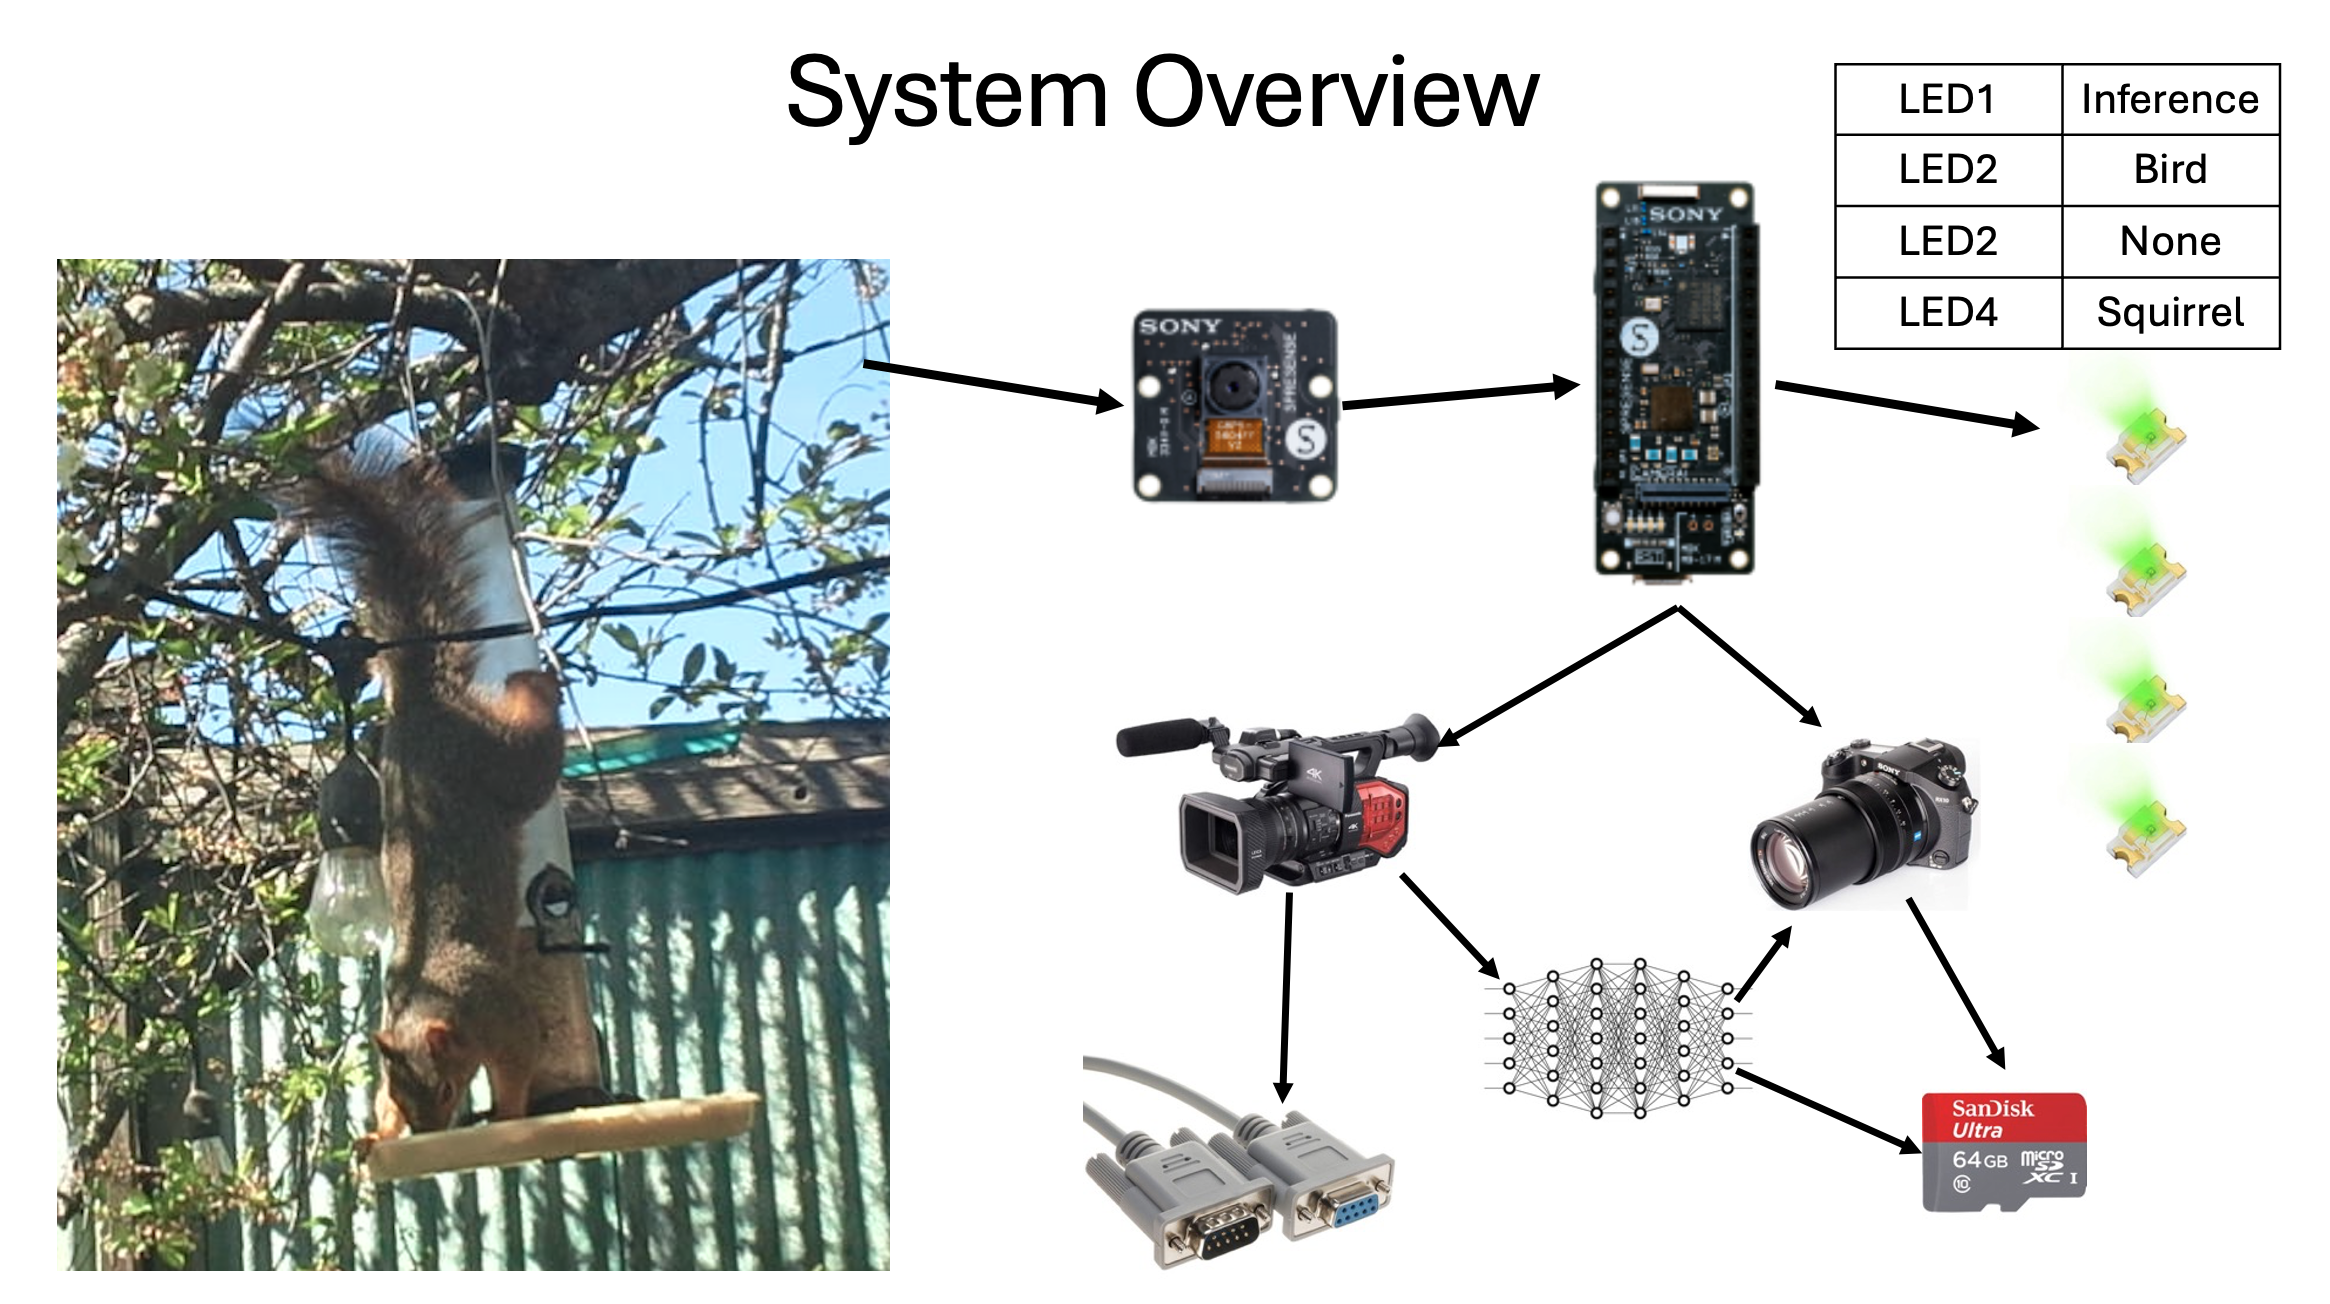
\includegraphics[scale=.22]{blockDiagram.png}}
\caption{System Diagram}
\label{blockDiagram}
\end{figure}


The system registers a callback to execute on video capture. This call back is set to the slowest speed available (5Hz).
The realtime data-flow is as follows:    
\begin{itemize}
     \item Capture the still immediately on the video callback.
     \item Center crop the video image to 96x96
     \item The cropped image is converted to RGB565
     \item The RGB image is converted to Float32 and normalized to 1.0
     \item The RGB656 is sent to TFLite inference
     \begin{itemize}
     	\item An LED is lit just prior to inference, and turned off at compleation
     \end{itemize}
     \item The results are interpreted as “Bird”, “Empty”, or “Squirrel”
     \item Light up the LED corresponding to the inference category
     \item If “Bird” or “Squirrel” (Or while gathering training data)
     \begin{itemize}
        \item The JPEG “still” is saved to an SD card
     \end{itemize} 
     \item A log file is written, with the inference results and save image number (-1 for no save)
     \item Send to serial Either:
     \begin{itemize}
        \item  Results, and tallies
        \item Cropped RGB565 image stream
        \end{itemize} 
\end{itemize} 

\begin{figure}[htbp]
\centerline{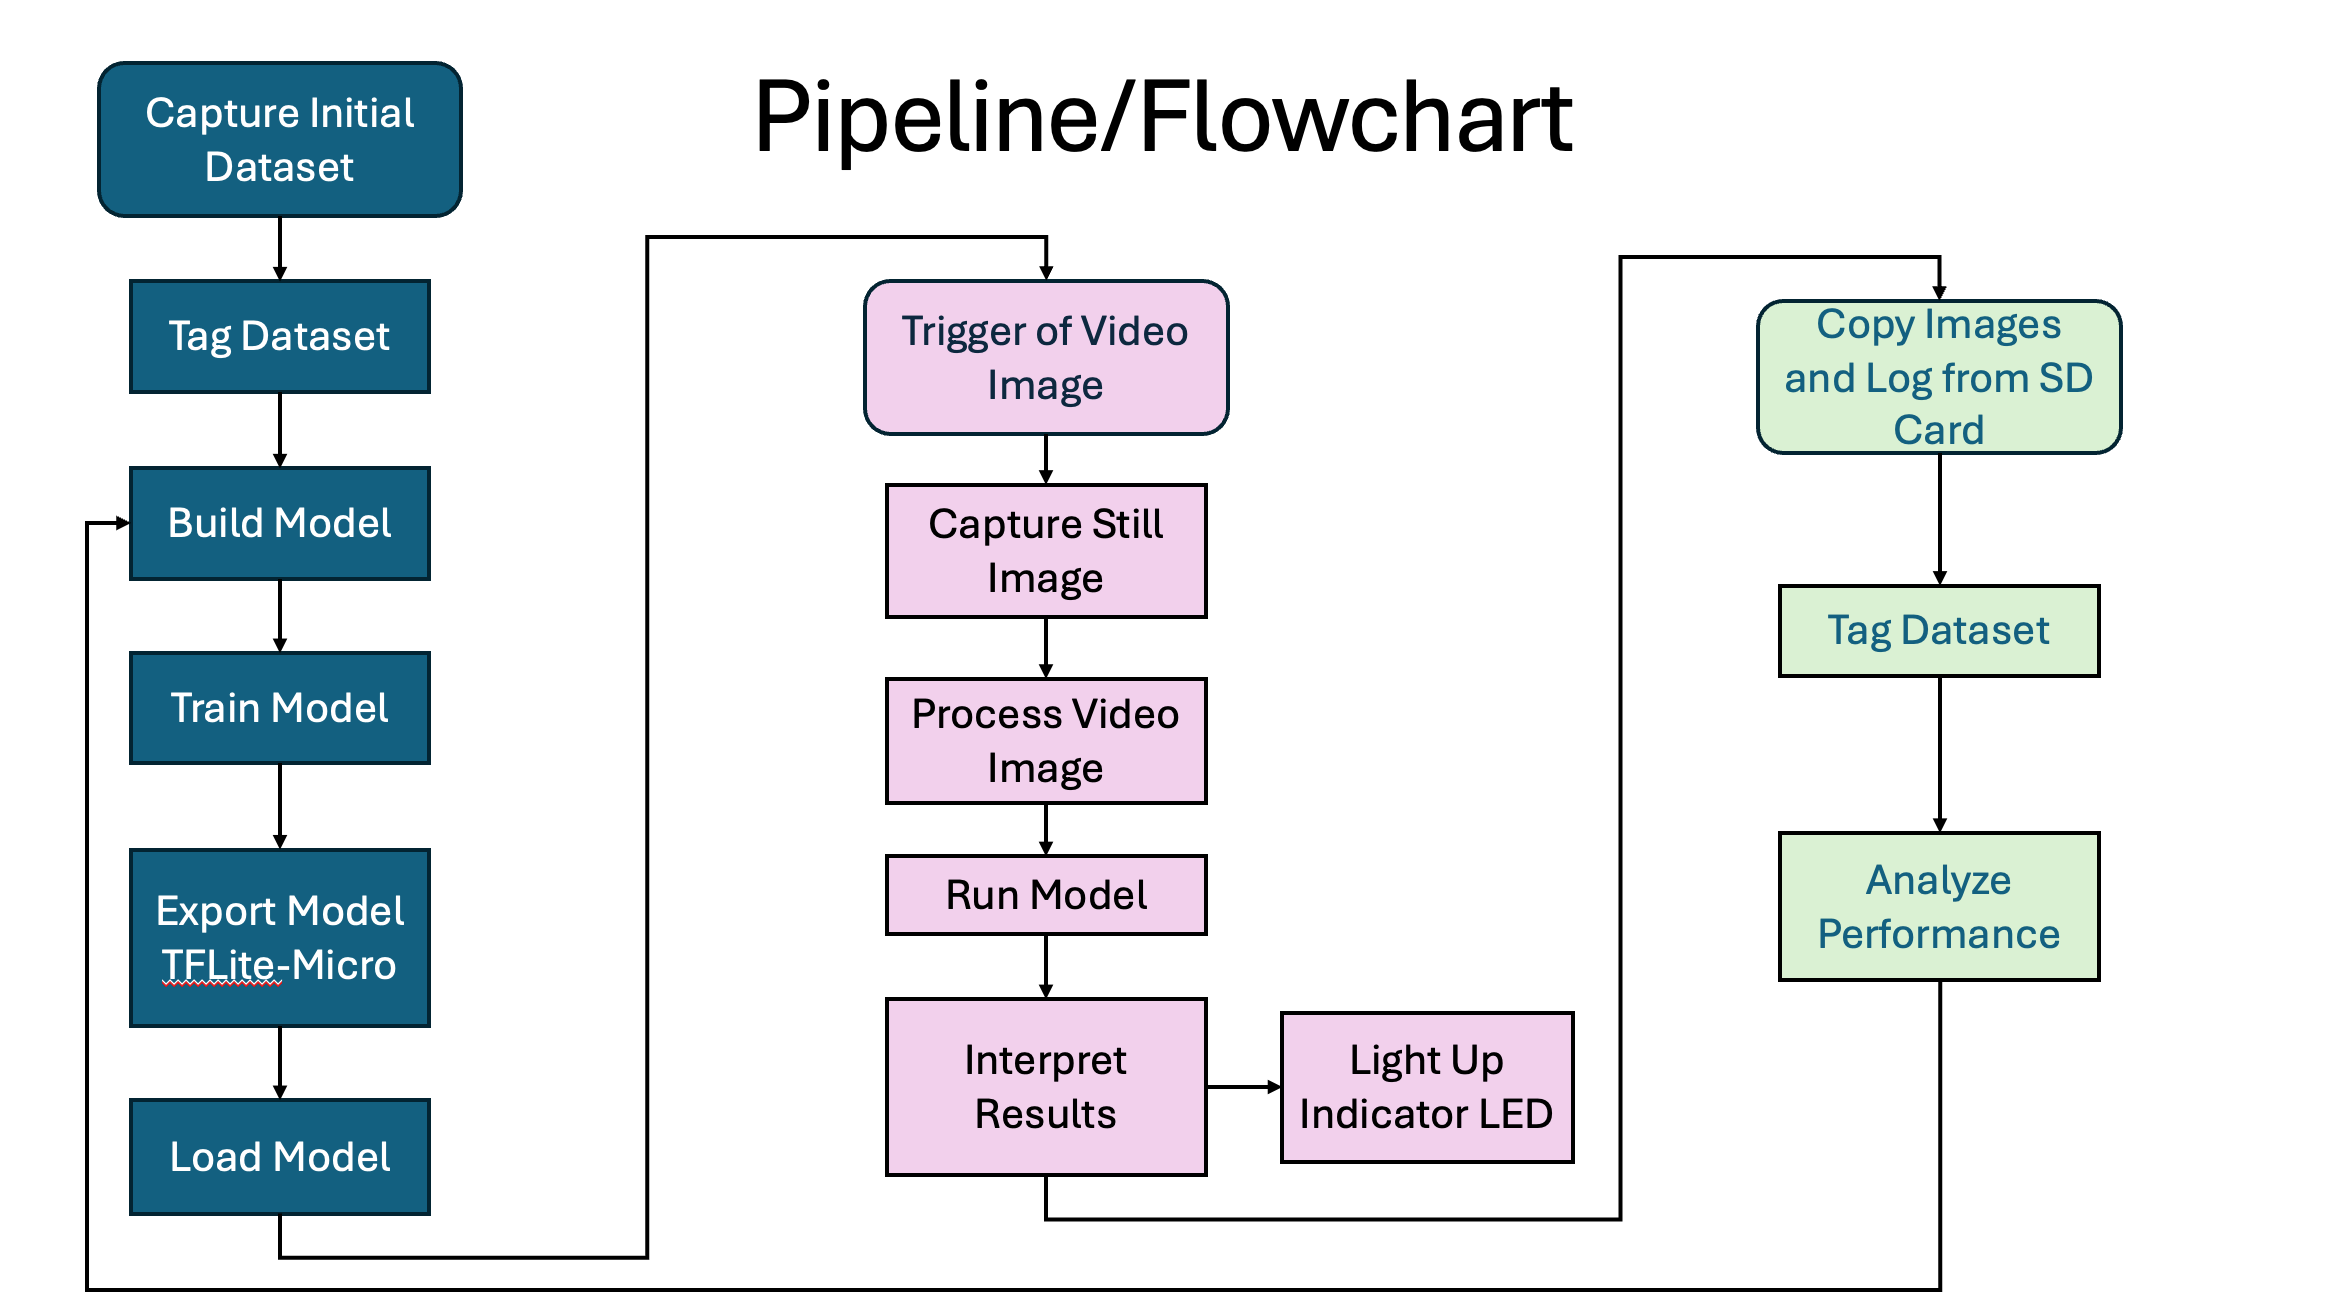
\includegraphics[scale=.22]{flowChart.png}}
\caption{Process Flow}
\label{flowChart}
\end{figure}

\subsection{Materials}

The system is built around a Sony Spresense CXD5602\cite{sony} Microcontroller. This microcontroller sits in a sweet spot of power, cost, and features. With a 6 core ARM M4F processor running at 156 MHz, and 1.5 MB of RAM, it has enough capabilities to run the required image processing and Machine Learning model. Yet it is low cost, and low power. The board only consumes 100mW (A Raspberry Pi 3B uses over 2W). The total hardware cost was less than \$200 `Table.~\ref{sysCost}''.

\begin{table}[htbp]
\caption{System Cost}
\begin{center}
\begin{tabular}{|c|c|c|c|}
\hline
\textbf{Component} & \textbf{\textit{Model}}& \textbf{\textit{Price (USD)}}   \\ \hline 
Microcontroller& Sony Spresense CXD5602 &   \$65\\ \hline 
Expansion Board& Sony Spresense Extension Board & \$45  \\ \hline
Memory Card& SanDisk 32GB Micro SD & \$20  \\ \hline
Camera& Sony Spresense Camera & \$35  \\ \hline
Tripod& Torjim Phone Tripod & \$10  \\ \hline
USB Cable& Micro USB A to Micro-B & \$3  \\ \hline
%\multicolumn{4}{l}{$^{\mathrm{a}}$Sample of a Table footnote.}
\end{tabular}
\label{sysCost}
\end{center}
\end{table}

\break
Microcontroller:
\begin{itemize}
	\item ARM Cortex-M4F @ 156 MHz
	\item SRAM: 1.5MB
	\item Power: 100mW
\end{itemize} 
Expansion Board:
\begin{itemize}
	\item SD Memory Card Slot
	\item 32GB High Speed SD Card
\end{itemize} 
Camera:
\begin{itemize}
	\item Image Transfer: CMOS 8-Bit Parallel
	\item Control interface: I2C
	\item Sensor: 2,608x 1,960 (~5 M pixel)
\end{itemize} 

\begin{figure}[htbp]
\centerline{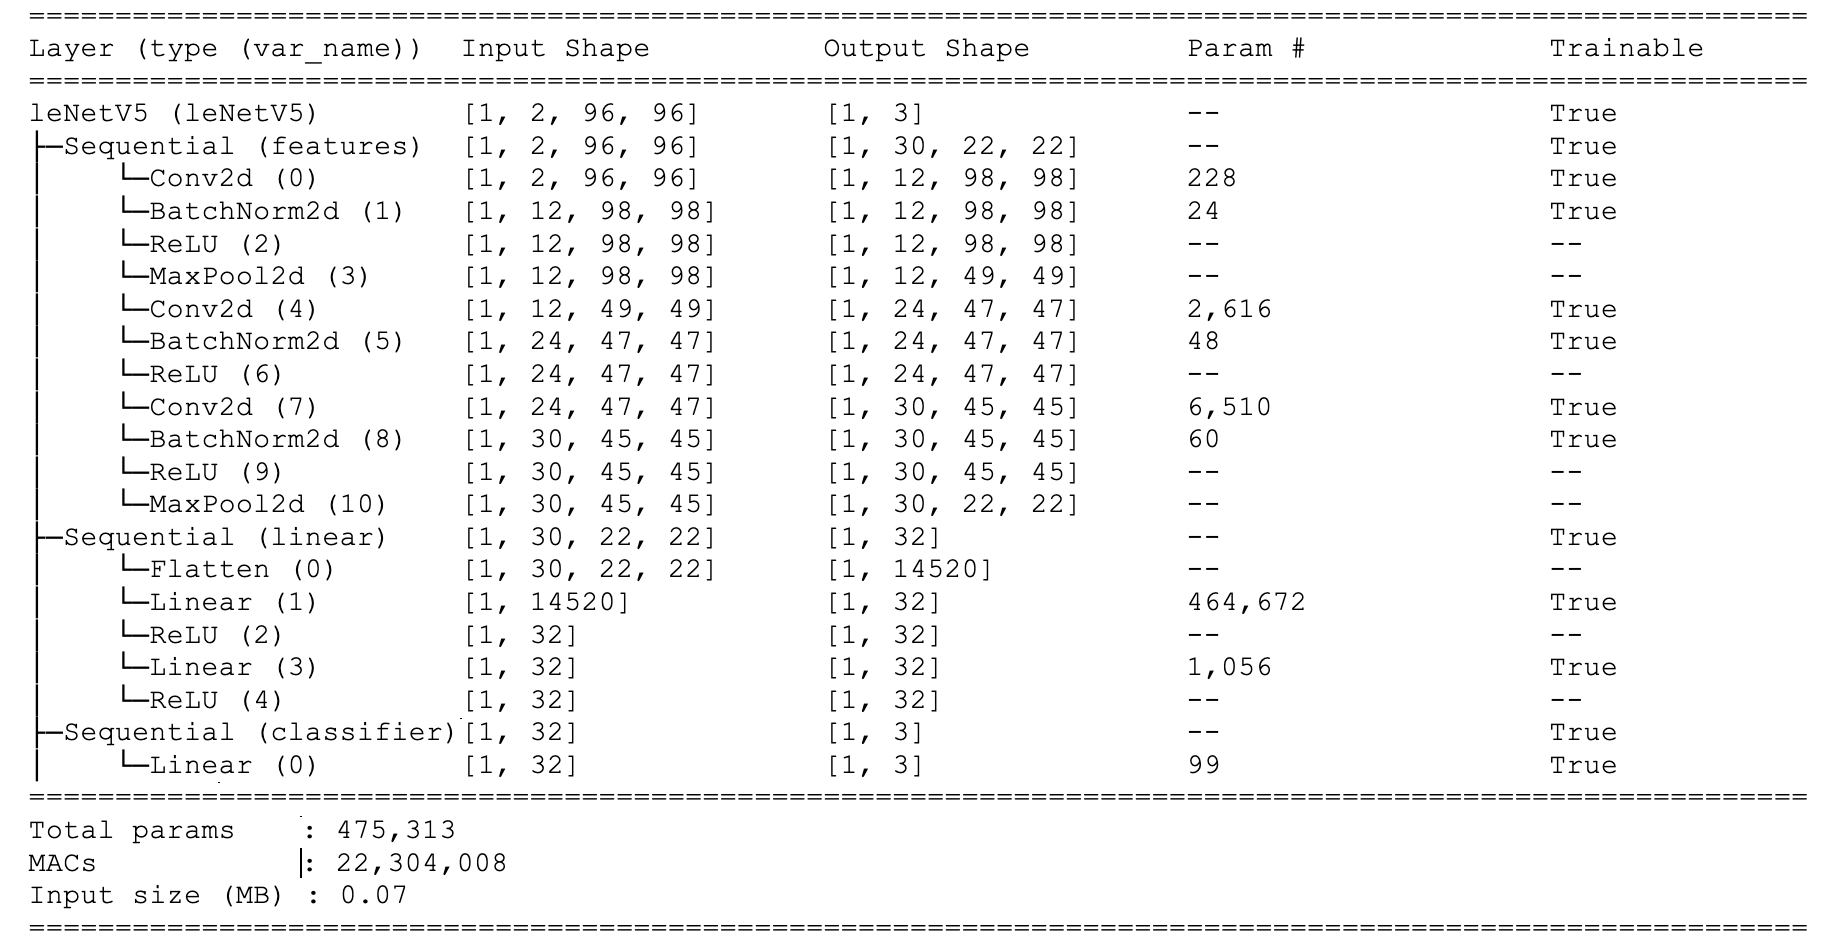
\includegraphics[scale=.22]{leNetV5.png}}
\caption{LeNetV5 Summary and Size}
\label{lenet}
\end{figure}

\subsection{Image Format}\label{AA}
The image format used as input to the model is RGB565. This is a three color bitmap format. 
Each color is stored is a 5-bit byte into 2 8 bit bytes ``Fig.~\ref{rgb565}''. RGB565 was selected for its 2 Byte bit depth and ease of use.
The image options available from the Sony Spresense Camera Library are:
\begin{itemize}
	\item RGB565
	\item YUV422
	\item JPEG
	\item Gray-scale
\end{itemize} 


\begin{figure}[htbp]
\centerline{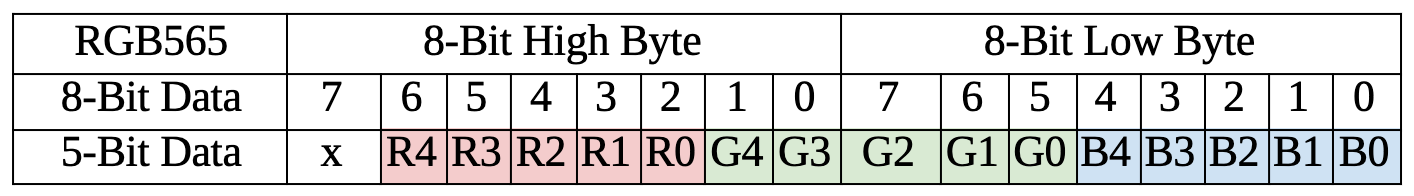
\includegraphics[scale=.22]{RGB565.png}}
\caption{RGB565 Byte Format}
\label{rgb565}
\end{figure}

\subsection{Training Procedure}

To train the model we first resize the training images to the largest image size we were able to use with the limited memory available. This was QVGA (320x240). The images are then center croped to the largest image size we were able to use while keeping the model small enough to fit. This is 96x96. Which is also the smallest size the Spresense camera library will crop to. The images are then converted to RGB565 and then converted to a PyTorch tensor. It is important to note that torchvision.transorms.ToTensor also converts the image data from UINT8 (0 to 255) to Float32 (0.0 to 1.0). This must be taken into account when running the model in realtime. Since we did not have a lot of images to work with, and the images were captured over a relatively small number of days and conditions, we augmented the image set using rotation and perspective distortion.  The number of "Empty" images also far outstretched the number of "Bird" and "Squirrel" images. The "Empty" images were randomly culled to bring the number of images in all classes somewhat the same for training and validation. Once we had achieved a good set of images, we successively trained and re-trained the model using a variety of hyperperamiters until we got a good training loss ``Fig.~\ref{tLoss}'". 


\begin{figure}[htbp]
\centerline{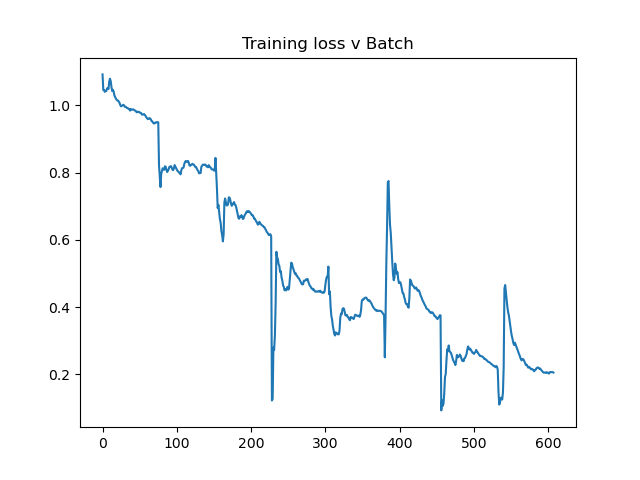
\includegraphics[scale=0.5]{trainingLoss.png}}
\caption{Training Loss}
\label{tLoss}
\end{figure}
The model was then run on the testing images and a confusion matrix generated ``Fig.~\ref{trainConfMat}'". This matrix is and images from poor performing categories are studied, the system is tweaked and re-run until we are happy(ish) with the performance.  The model is then loaded onto the microcontroller, and the camera is setup to capture images of the feeder for a day. These images are manually tagged, and run the performance analyzed. The model is then re-tweeked, and retrained on the growing image set. Wash, rinse, repeat. An example training validation confusion matrix `Fig.~\ref{trainConfMat}''.
\begin{figure}[htbp]
\centerline{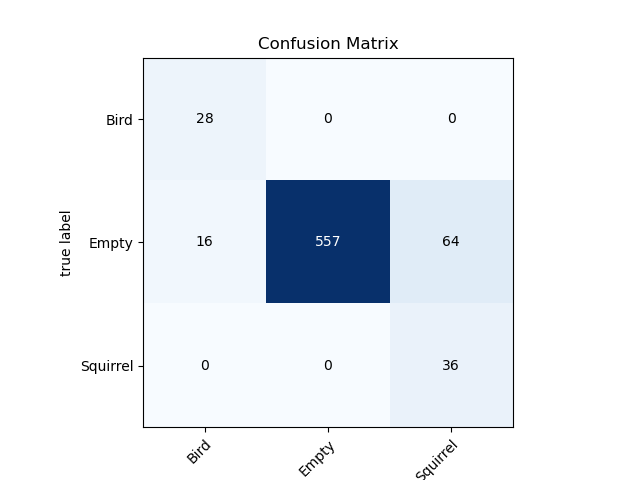
\includegraphics[scale=0.4]{trainValConfMat.png}}
\caption{Training Validation Confusion Matrix}
\label{trainConfMat}
\end{figure}

\begin{itemize}
	\item Image Conversion
	\begin{itemize}
		\item Resize to QVGA 320x240
		\item Center Crop to 96x96
		\item Convert to RGB565
		\begin{itemize}
			\item Byte swap R and B
		\end{itemize}
		\item Convert images ToTensor
	\end{itemize}
	\item Image augmentation
	\begin{itemize}
		\item For each bird and squirrel make a copy that is
		\begin{itemize}
			\item Randomly rotated -10 to 10 degrees
			\item Randomly perspective distorted up to 25\%
		\end{itemize}
		\item For Empty
		\begin{itemize}
			\item Cull image set to same numbers and augmented birds and squirrels
		\end{itemize}
	\end{itemize}
	\item The final hyperparameters of the  LeNetV5 \cite{leNet} Model are summarized in ``Table.~\ref{hyperparameters}''.
\end{itemize}

\begin{table}[htbp]
\caption{Model Training Hyperparameters}
\begin{center}
\begin{tabular}{|c|c|c|c|}
\hline

\textbf{Hyperparameter} & \textbf{\textit{Value}}    \\ \hline 
Epochs& 8 \\ \hline 
Learning Rate& 0.01 \\ \hline 
Batch Size& 16 \\ \hline 
Criterion& Cross Entropy Loss \\ \hline 
Optimizer& SGD \\ \hline 
\end{tabular}
\label{hyperparameters}
\end{center}
\end{table}


\subsection{Installing Model on MicroController}
One of the more complex procedures is the converting and installing of the machine learning model into the resource limited microcontroller. The first step in this process is to determine how large a model and image size can fit onto the selected microcontroller. Our board has 1.5MB to work with, and this space must be shared between the model, the images, the software (Including the Tensor Flow Lite library set), as well as the base operating system, and the memory space required to run the model (The Arena Size).  These sizes are all interdependent on each other and some must be iteratively determined ``Table.~\ref{memUse}''.
\begin{table}[htbp]
\caption{Quantization Sumary}
\begin{center}
\begin{tabular}{|c|c|c|c|}
\hline
\textbf{Item} & \textbf{\textit{Size (kB)}}    \\ \hline 
	Camera Image & 154\\ \hline
	Save Image & 50\\ \hline
	Model Image &  18 \\ \hline 
	Model& 482 \\ \hline 
	Arena& 166 \\ \hline 
	Libraries, Program and OS & 67\\ \hline 
	 & \\ \hline
	 Memory Installed & 1,573 \\ \hline
	 Total Used& 938 \\ \hline
\end{tabular}
\label{memUse}
\end{center}
\end{table}

Once the model is built and trained it is converted to TensorFlow Lite for Microcontrollers ``Fig.~\ref{torch2tf}'' then installed on the microcontroller.
\begin{itemize}
	\item Convert the model to ONNX using torch.onnx
	\begin{itemize}
		\item Required input:  Image Shape (2x96x96)
	\end{itemize}
	\item Convert the ONNX file to TensorFlow using onnx2tf
	\begin{itemize}
		\item Required input:  mean and standard deviation of training image set by pixel
	\end{itemize}
	\item Export the TensorFlow file to TensorFlow Lite
	\begin{itemize}
		\item Quantization of the model from 32 Bit Float to 8 Bit Int is done at this step.
	\end{itemize}
	\item Hex dump the TensorFlow Lite file using xdd to save as a c header
	\begin{itemize}
		\item shell: xxd -i leNetV5.tflite \textgreater leNetV5
	\end{itemize}
\end{itemize}

\begin{figure*}[htbp]
\centerline{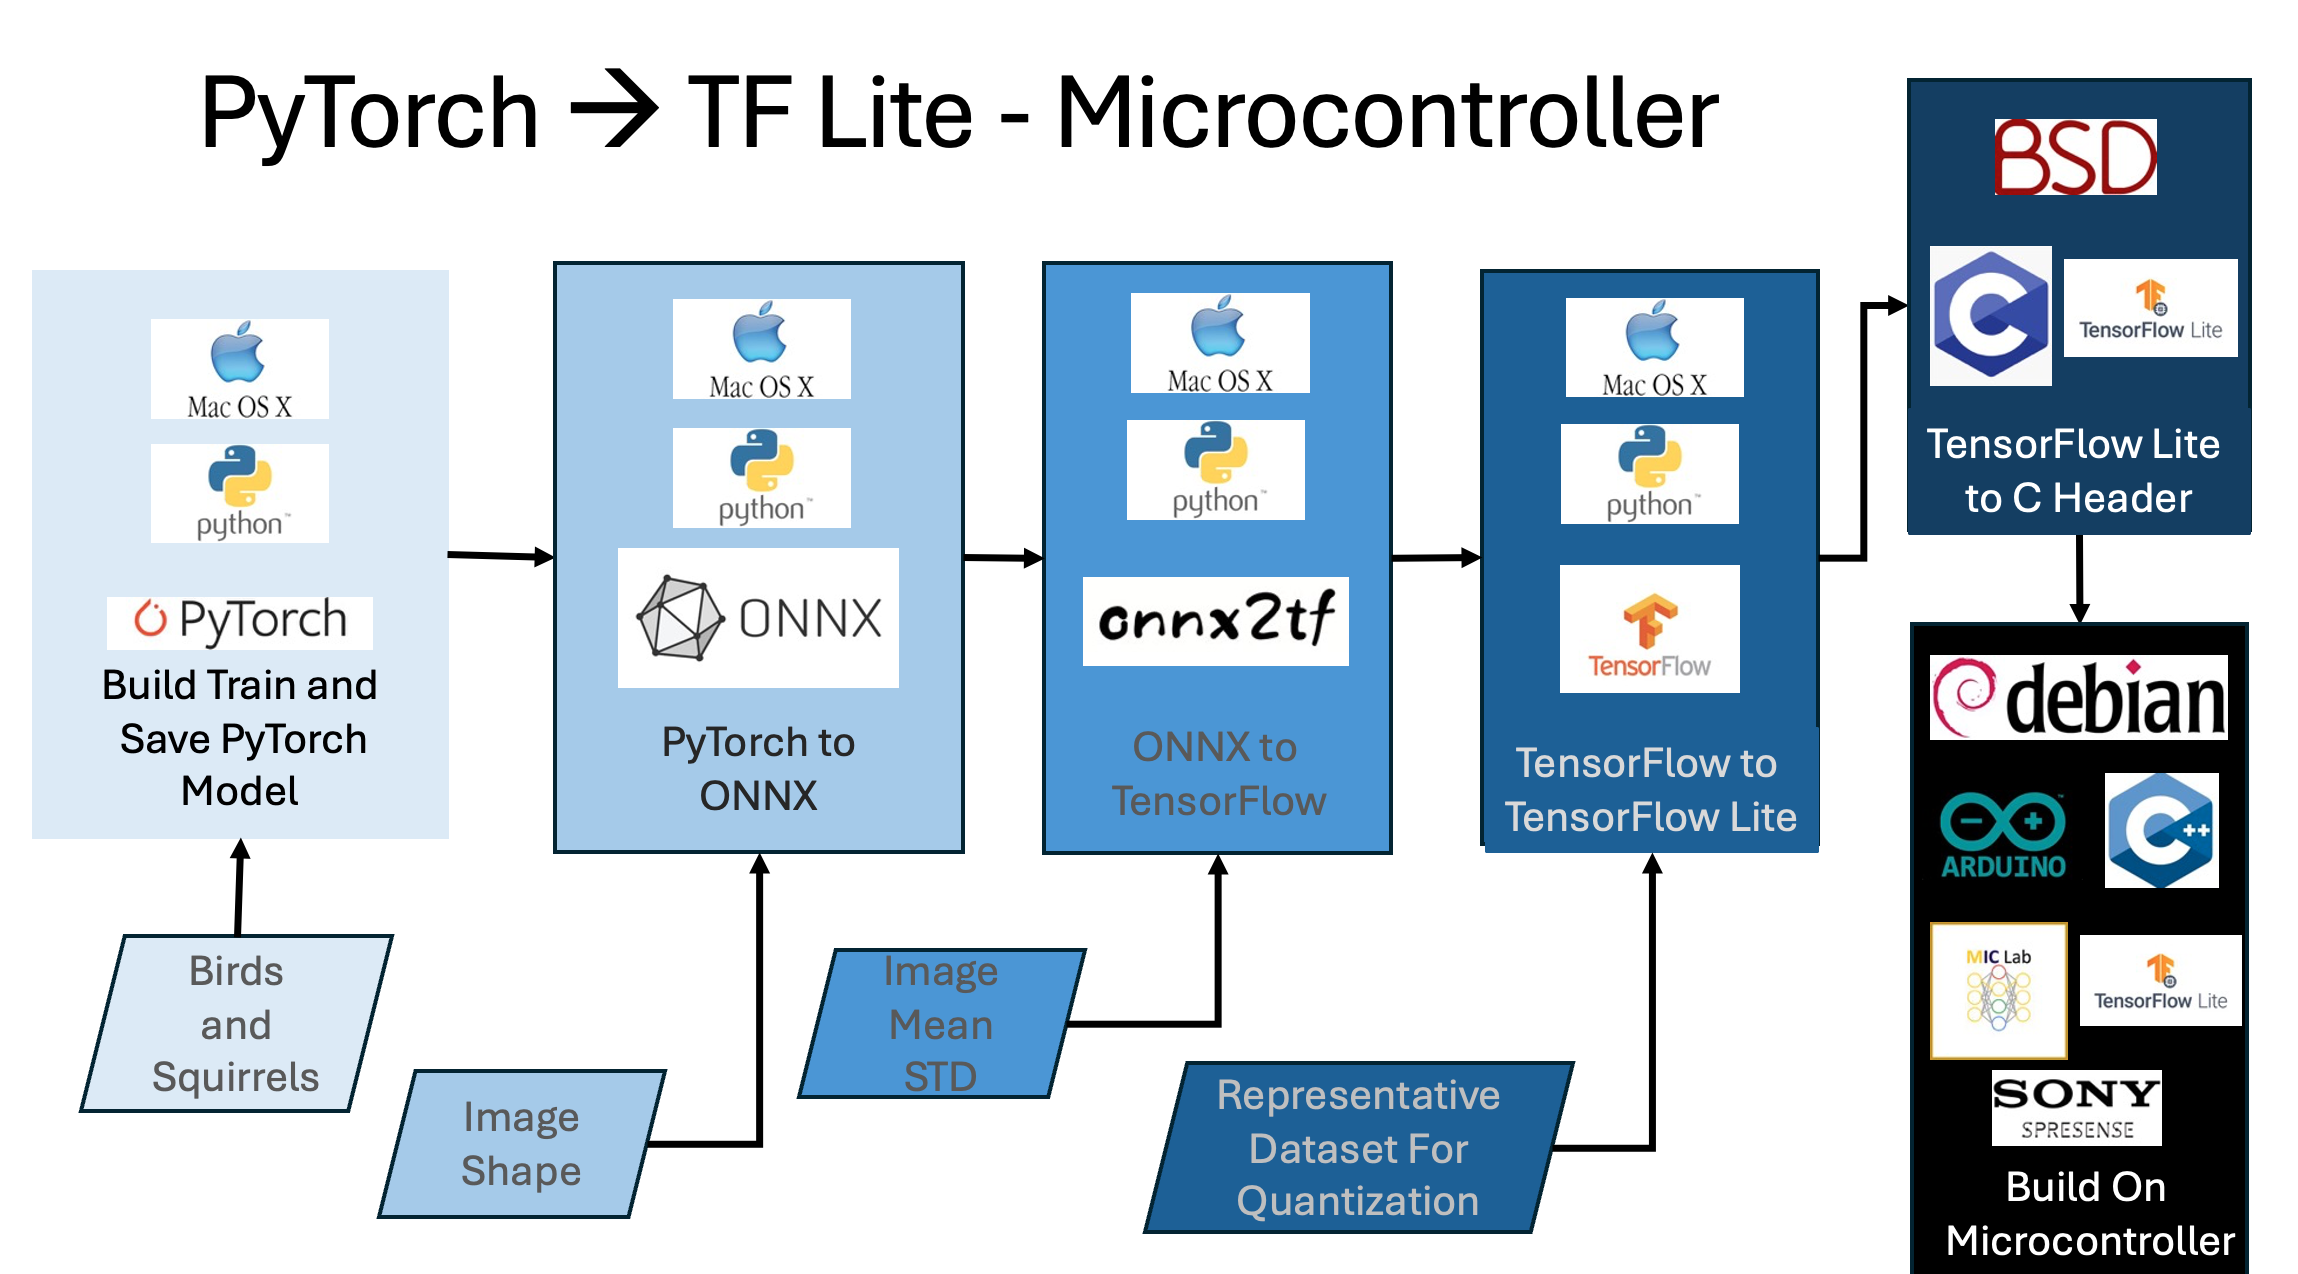
\includegraphics[scale=0.3]{pyTorch2TFLite.png}}
\caption{PyTorch --\textgreater Tensor Flow Lite Workflow}
\label{torch2tf}
\end{figure*}

\begin{table}[htbp]
\caption{Quantization Sumary}
\begin{center}
\begin{tabular}{|c|c|c|c|}
\hline
\textbf{Quantization} & \textbf{\textit{Size (kB)}}    \\ \hline 
	Float 32& 1,961 \\ \hline 
	Float 16& 956 \\ \hline 
	INT 8& 482 \\ \hline 
\end{tabular}
\label{quantSum}
\end{center}
\end{table}

During the conversion process the model is also quantized. As ``Table.~\ref{quantSum}'' shows, quantizing to INT8 is critical to get the model small enough to fit on the limited (1.5MB) memory space of the microcontroller.
The model size + the input image size is 18 kB + 482 kB = 500 kB. It may be tempting to look at the table and think that we can use Float 16, rather than INT 8, however this change would also require an increase in Arena size. Similarly one might be tempted to increase the models image size to QQVGA (160x120) as that would only bring 20kB more. However this would increase the model size, also requiring a larger arena. The domino effect would be an addition of more than the 600kB available space. Further complicating the process, if we went much  over  90\% memory usage the board would not boot. 

\begin{table}[htbp]
\caption{Training Image Counts}
\begin{center}
\begin{tabular}{|c|c|c|c|}
\hline
\textbf{Classification} & \textbf{Training Images}   & \textbf{Validation Images} \\ \hline 
	Bird& 195 & 25\\ \hline 
	Empty& 467 & 89\\ \hline 
	Squirrel& 549 & 61\\ \hline 
\end{tabular}
\label{numImages}
\end{center}
\end{table}

\section{Results}\label{SCM}
Once everything was functional, and a training set with fairly good validation numbers was achieved ``Fig.~\ref{trainConfMat}'" the system was set up to perform a realtime run. The results of the initial Real Time Run Confusion Matrix `Fig.~\ref{rt1ConfMat}'' were pretty good for squirrel and Empty, but disappointing for detection of birds.  The model was subsequently re-trained including the images gathered on the first successful run. After retraining on larger image set Real Time Run Confusion Matrix `Fig.~\ref{rt2ConfMat}''. This proved very successful in determining positive hits on the "Empty" case. However, this progress came at the cost of poor performance in the "Squirrel" case. The detection of "Bird" also remained poor.
\begin{figure}[htbp]
\centerline{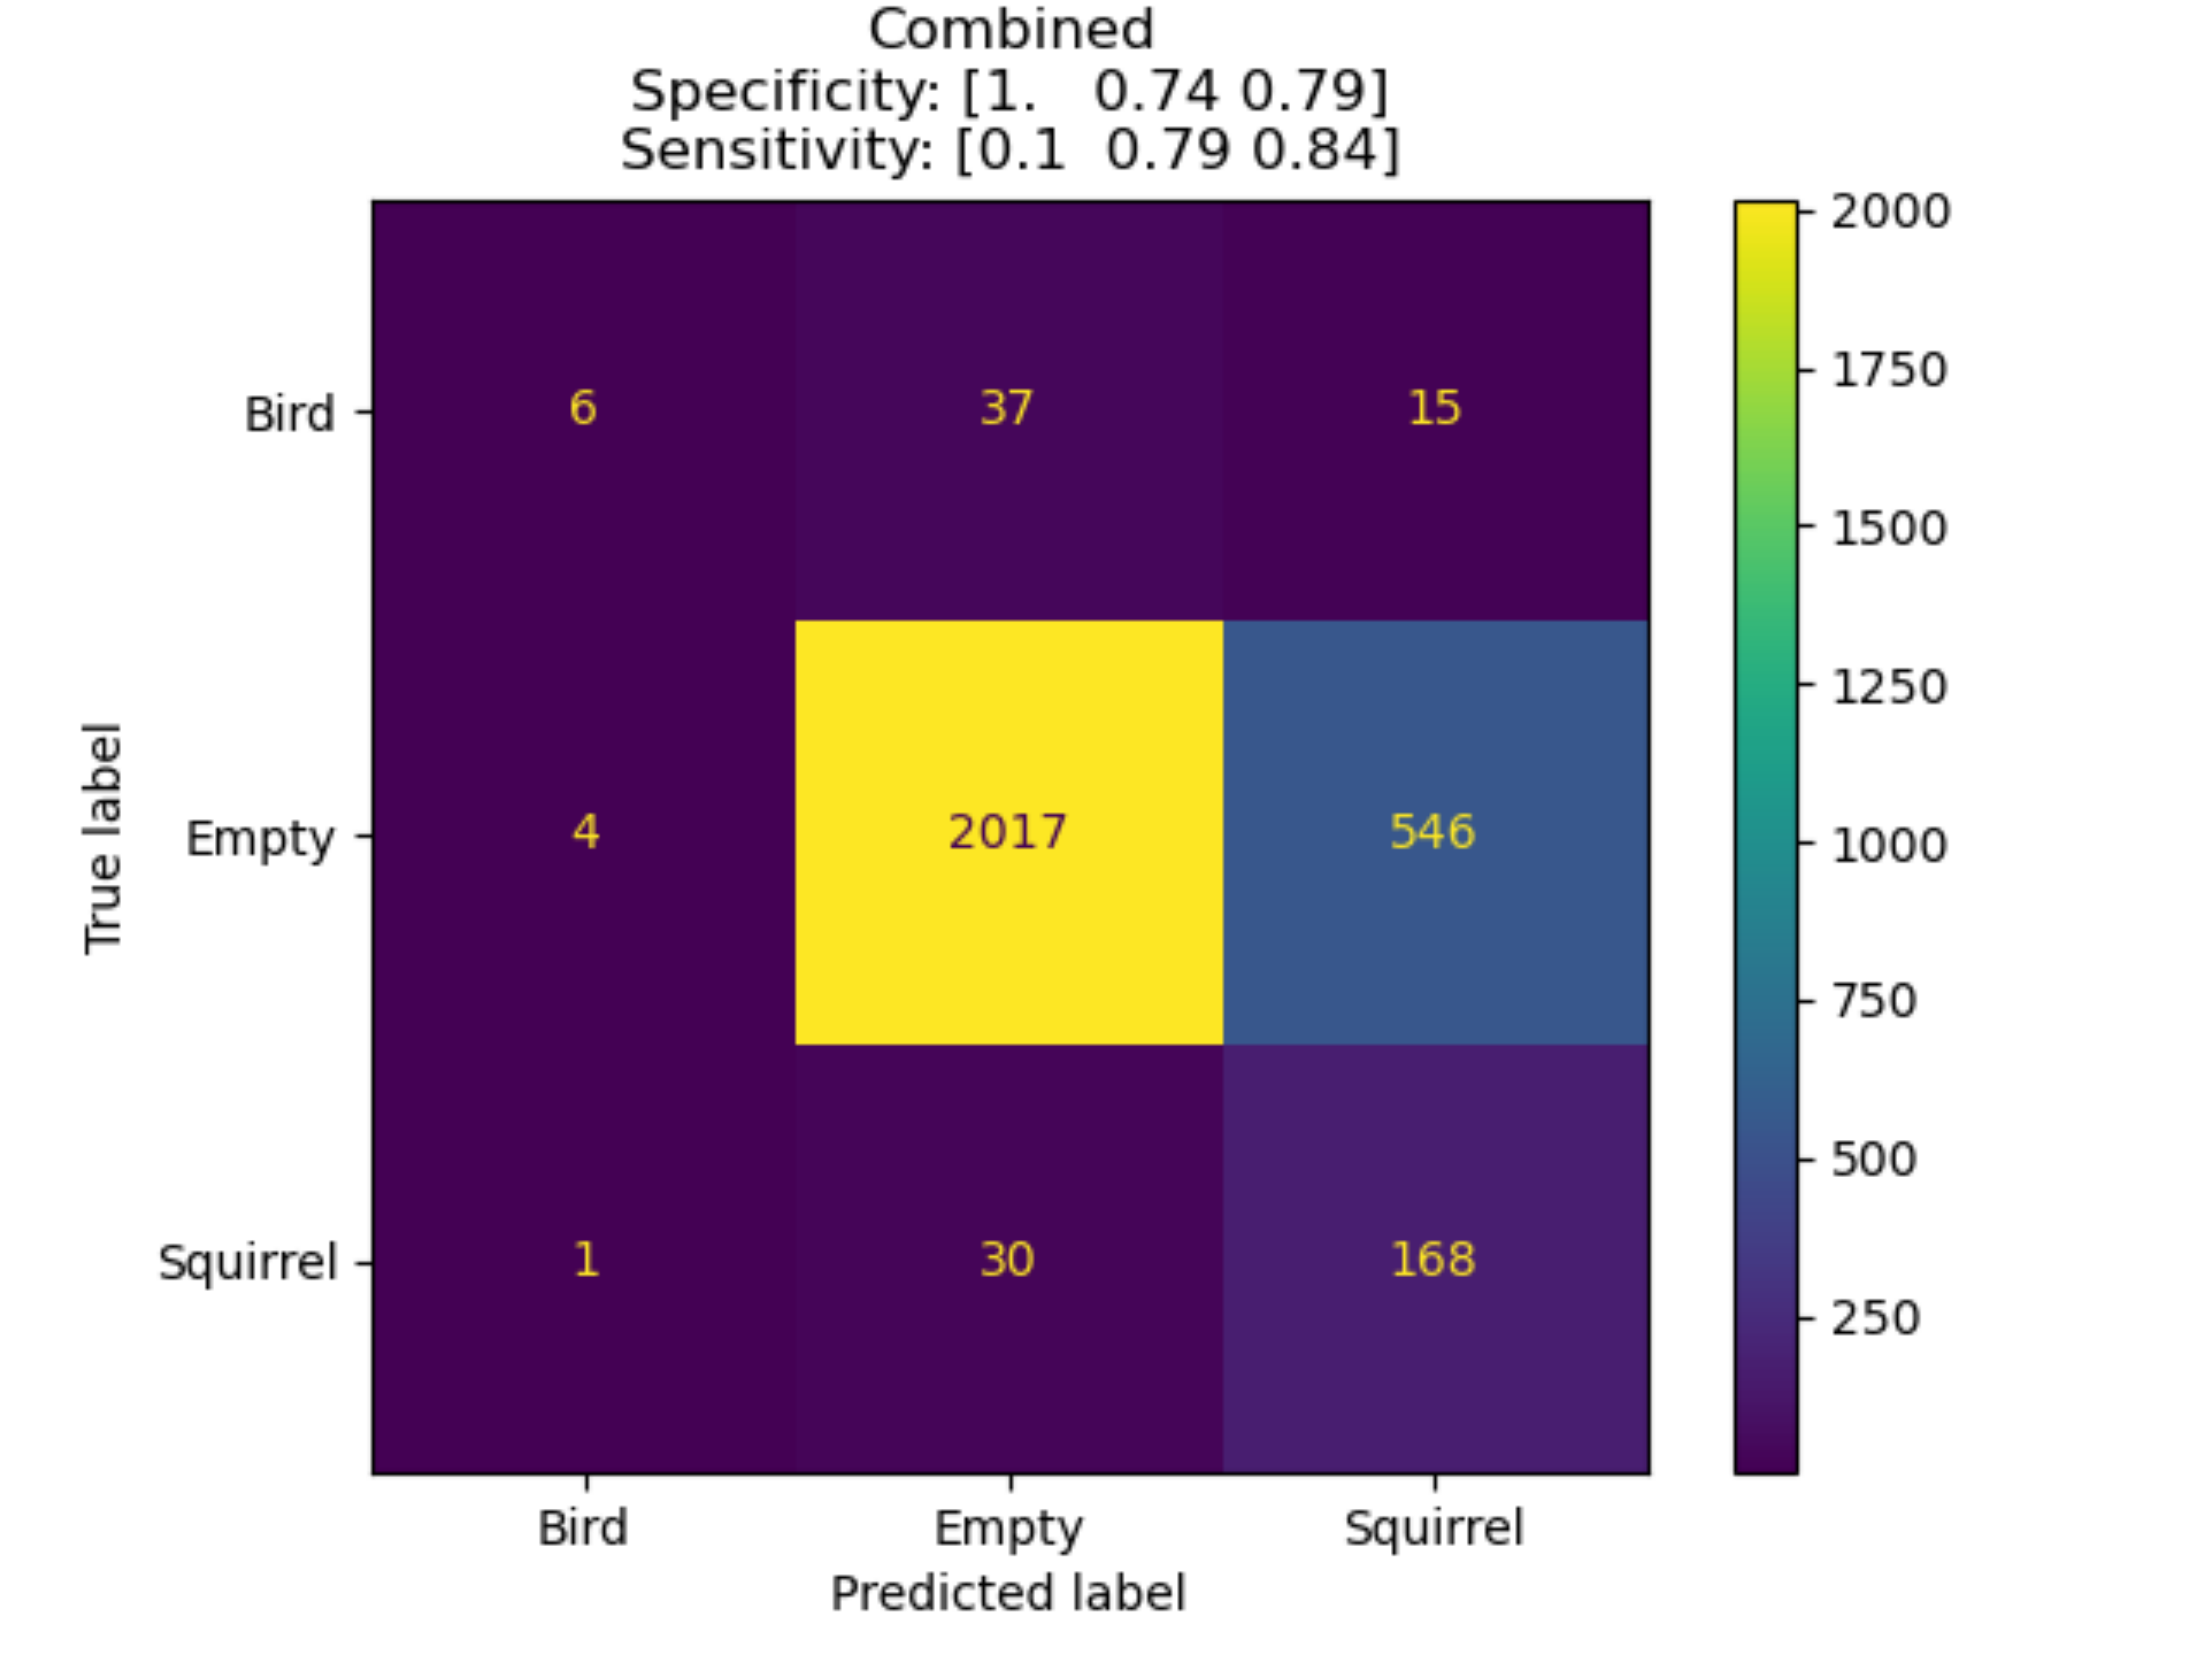
\includegraphics[scale=0.06]{initialRunConfMat.png}}
\caption{Initial Real Time Run Confusion Matrix}
\label{rt1ConfMat}
\end{figure}
\begin{figure}[htbp]
\centerline{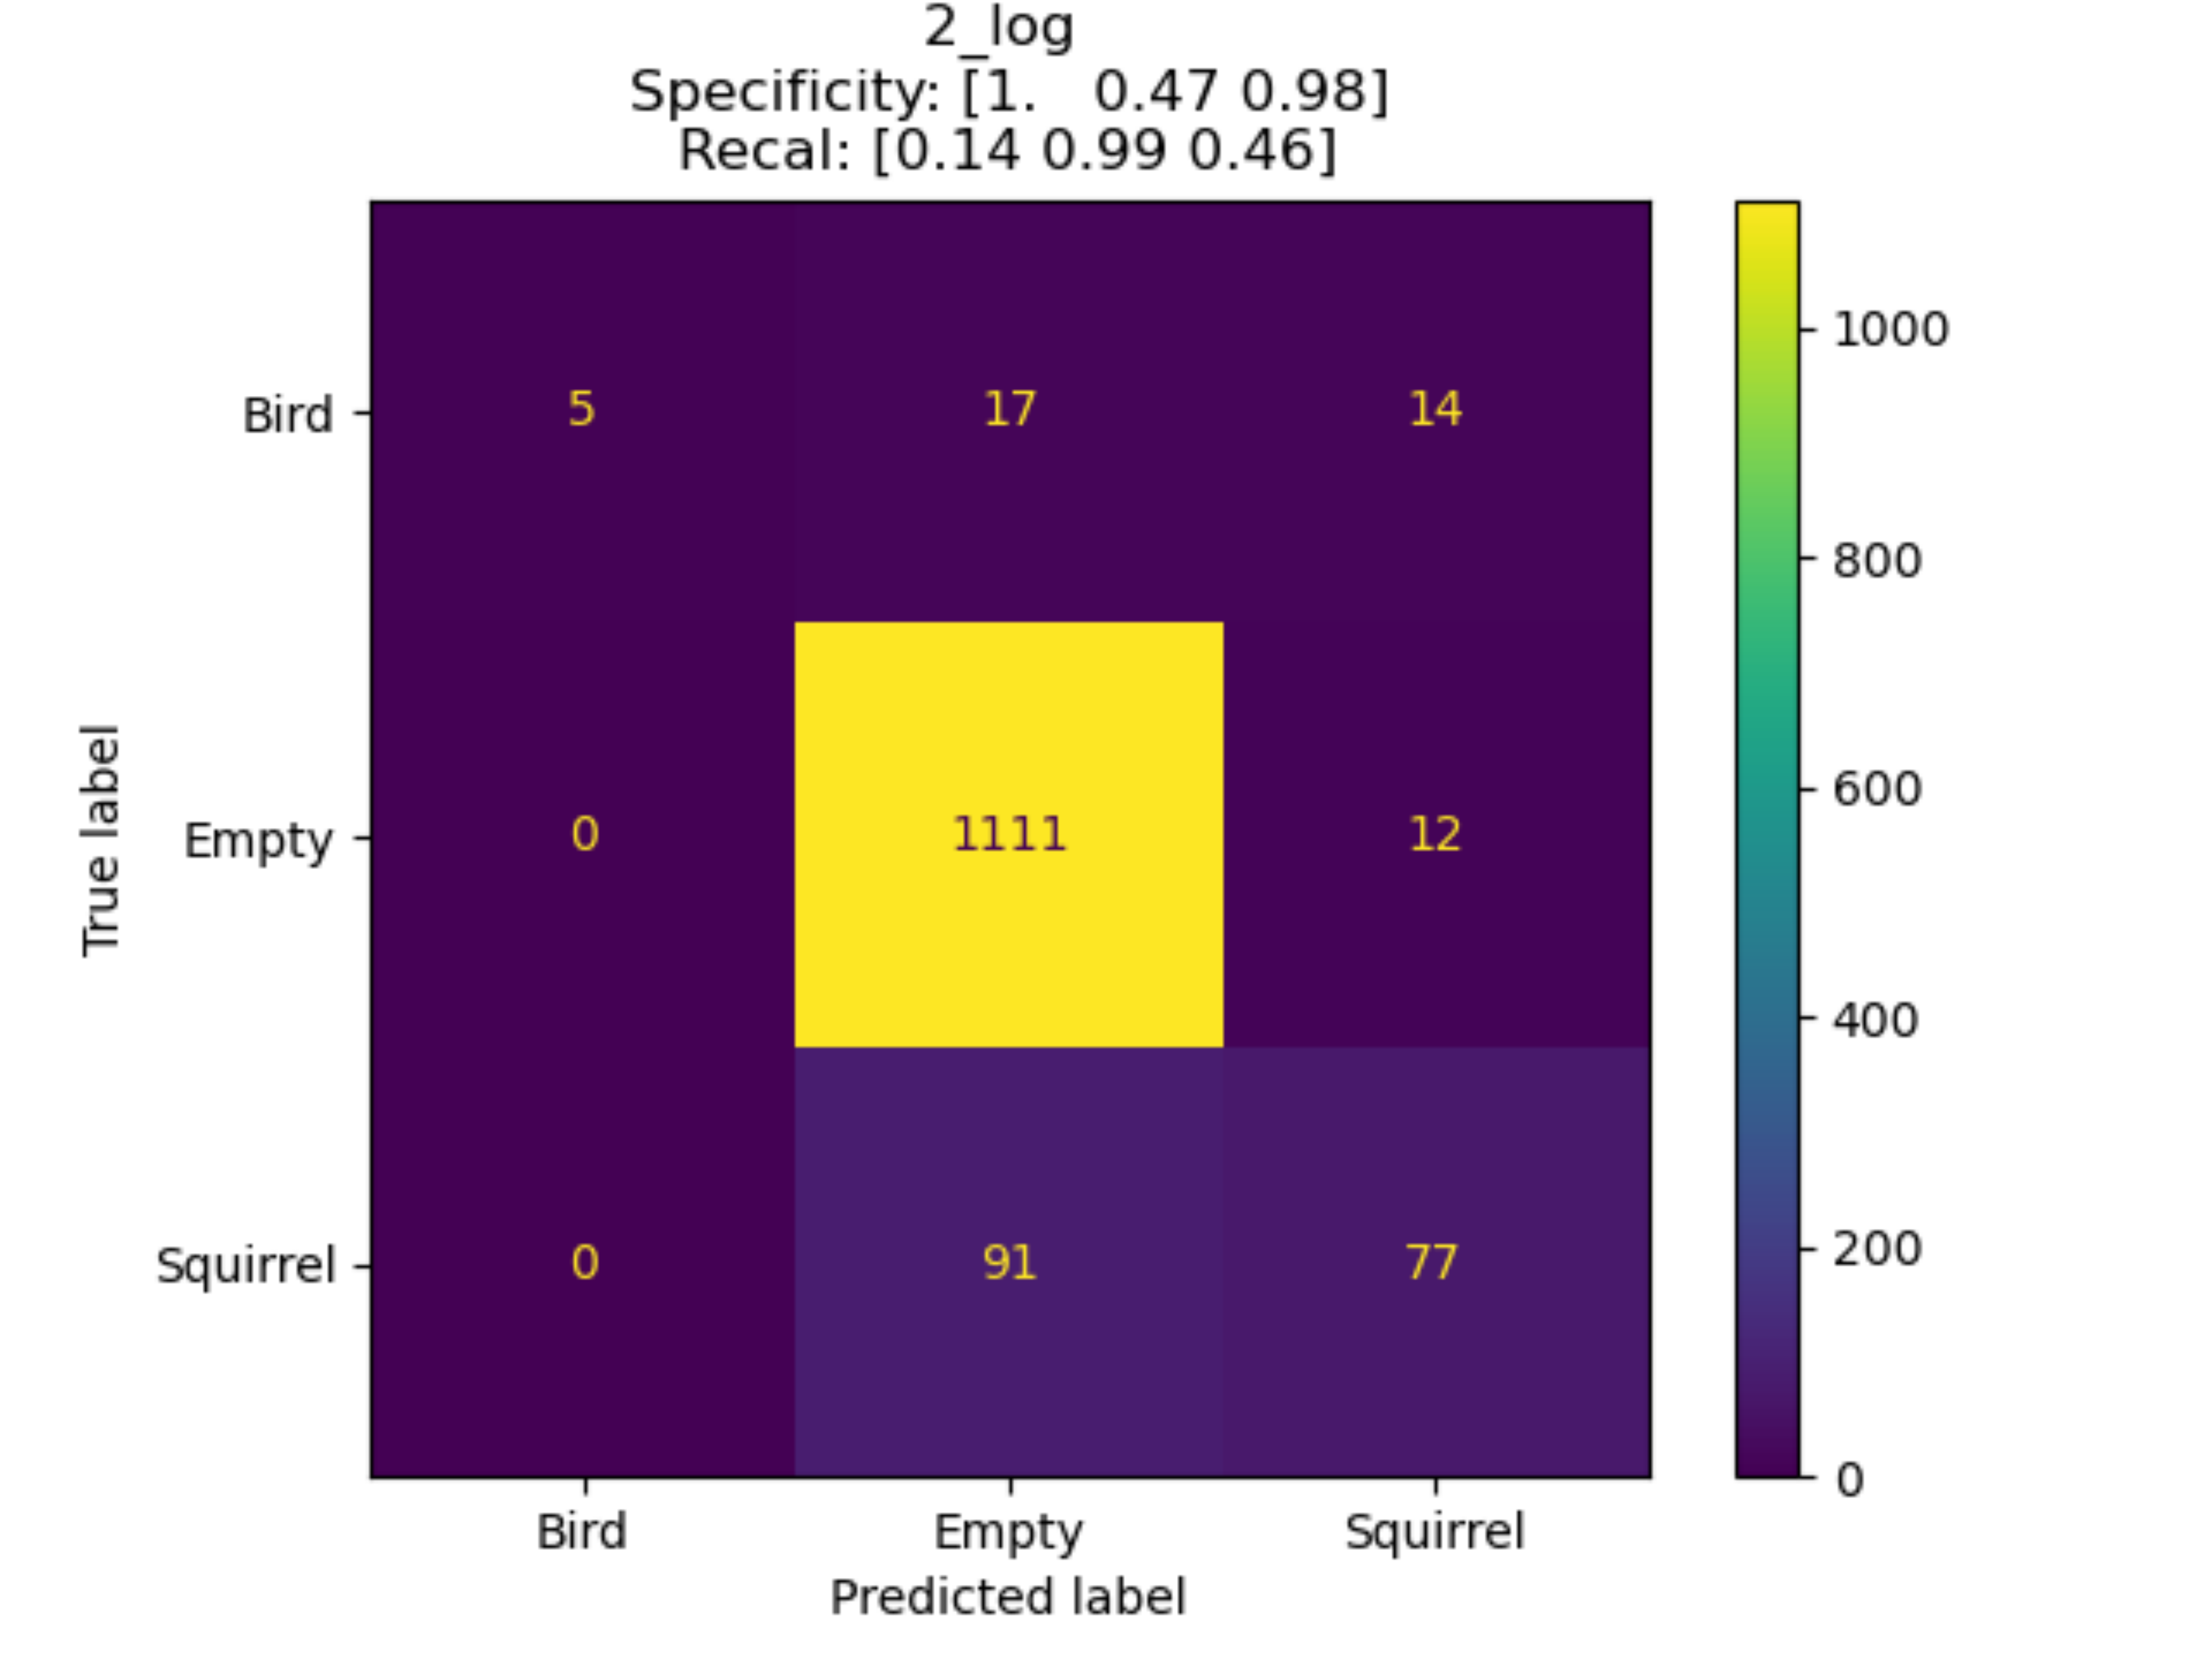
\includegraphics[scale=0.06]{afterReTrainConfMat.png}}
\caption{After retraining on larger image set Real Time Run Confusion Matrix}
\label{rt2ConfMat}
\end{figure}
After analyzing the images that were successful and unsuccessful in determining "Bird", the reason was discovered ``Fig.~\ref{sBirdbBird}''. It turns out that once the images are cropped to 96x96, the small birds are almost indistinguishable from no bird. Another major factor in the overall system performance is the lack of training images ``Table.~\ref{numImages}''. These counts are very small, even when image augmentation was used. We made a decision to only use a few days worth of images for the final training due to a storm that had come in and radically rearranged the tree branches that the feeders were hanging from.\\
\begin{figure}[htbp]
\centerline{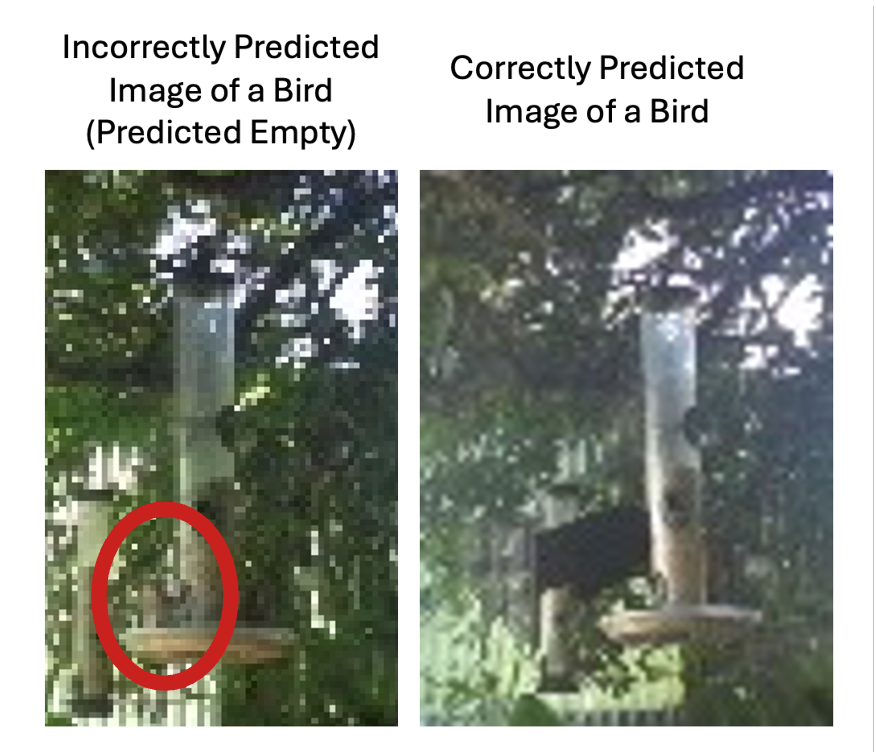
\includegraphics[scale=0.5]{wongBirdRightBird-2.png}}
\caption{Incorrect (small) Bird. Correct (Large) Bird.}
\label{sBirdbBird}
\end{figure}
The performance of the system can be improved by using a larger image size and by training on a much larger image set. If a larger image size proves impossible due to memory space limitations, then the "Bird" focus should be limited to larger birds. (e.x. Blue Jay, Mourning Dove, and Crows: All of which are daily visitors). The singular goal of the system is the detection of the Squirrels, the bird detection is secondary, and most useful in avoiding false positive hits for squirrels.\\
One final note, is that the inference time is long. With the model as build it takes 20 seconds to run. This, while extraordinarily long, is not detrimental to the detection of squirrels, as when they do come, they will stay for many minutes at a time. However, we believe that the inference time can be dramatically improved by switching the LeNetV5 model to a MobileNetV1. However, the MobileNetV1 model trained on the 2x96x96 image set is 71.2MB in PyTorch, 18MB after quantization and converting to Tensor Flow Lite. The initial MobileNetV1, however, does show promising initial results ``Fig.~\ref{MbNetV1ConfMat}''. The size can be remedied by vastly trimming the layer count and size of each layer. The performance can be further improved by increasing the number of training images, augmentation, and tweaking the hyperparameters.\\
\begin{figure}[htbp]
\centerline{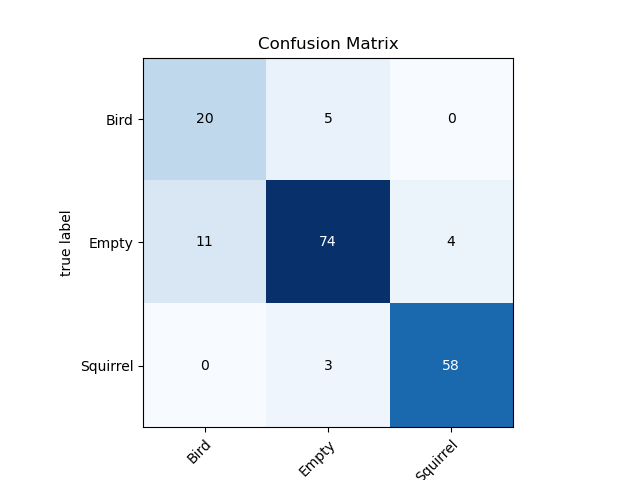
\includegraphics[scale=0.5]{MbNet_confMatrix.png}}
\caption{MobileNetV1 Confusion Matrix}
\label{MbNetV1ConfMat}
\end{figure}
Once the system is performing better the final step will be to waterproof, and use a water jet to deter the squirrel once detected.




\begin{table*}[htbp]
\caption{Summary of Code Base}
\begin{center}
\begin{tabular}{|c|c|c|c|}
\hline
\textbf{Module} & \textbf{Hardware/OS/Platform}  &\textbf{File}  &\textbf{Language}\\ \hline 
	RealTime & Sony Spresense/Arduino & sqVB1rd\_ard.ino & C++ \\ \hline
	RealTime Model & TensorFlow Lite & RGB2BGRleNetV5\_trained.h & C Header \\ \hline
	RealTime Serial Image Diaplay & Processing: https://processing.org & processingScript.pde & Java \\ \hline
	Image Capture/First Attempt at RealTime & Sony SpreSense/SDK & \begin{tabular}[x]{@{}c@{}} sqb\_main.c, camera.c, camera.h,\\ cardUtils.c, cartdUtils.h, DSC.config \end{tabular}    & C \\ \hline
	Data Augmentation &  torchvision & DataAugment.py & Python \\ \hline
	Image Loading & TorchVision & DataPreparation.py & Python \\ \hline
	Convert Image & CV2 & BGR2RGB565.py\cite{MIC} & Python \\ \hline
	Rename Images & OS & fileOpps.py & Python \\ \hline
	Model Training & PyTorch & main.py & Python \\ \hline
	Model Training & PyTorch & Model.py & Python \\ \hline
	Model Definition & PyTorch & Trainer.py & Python \\ \hline
	Model Converting & `Fig.~\ref{torch2tf}'' & saveModel.py & Python \\ \hline
	Model Optimization & MIC Pruning Engine & optimize.py & Python \\ \hline
	Model Validation & Tensor Flow & RunTfLite.py & Python \\ \hline
	Model Validation & PyTorch & validate.py & Python \\ \hline
	Data Analysis & Torch Metrics/SSklearn & analysis.py & Python \\ \hline
	Model Analysis & thop & OpCounter.py & Python \\ \hline
\end{tabular}
\label{codeSum}
\end{center}
\end{table*}

\begin{thebibliography}{00}

\bibitem{king}  King Nicola, Sadowski, (2001) ML-based Bird and Squirrel Detector, MagPi, https://magpi.raspberrypi.com/articles/ml-based-bird-and-squirrel-detector
\bibitem{mary}  T. Mary. (2021). Solving the Problem of Squirrels Stealing from the Bird feeder: Prototyping Image Classification with the Deep Learning Workbench in Intel® DevCloud for the Edge. Intel Community, https://community.intel.com/t5/Blogs/Tech-Innovation/Artificial-Intelligence-AI/Solving-the-Problem-of-Squirrels-Stealing-from-the-Bird-feeder/post/1335676
\bibitem{chap} Chapman, J. B. (1996). Effectiveness of capsaicin as a squirrel repellent at bird feeders. Mississippi State University.
\bibitem{krause} Krause, S. K., Kelt, D. A., \& Van Vuren, D. H. (2010). Invasion, damage, and control options for eastern fox squirrels. In Proceedings of the Vertebrate Pest Conference (Vol. 24, No. 24). 

\bibitem{sony} Sony. (2004). Sony Spresense Specifications. https://developer.sony.com/spresense/product-specifications 
\bibitem{MIC} MIC Lab. (2024). http://sfsu-miclab.org/ 
\bibitem{singla} Singla, N. (2014). Motion detection based on frame difference method. International Journal of Information \& Computation Technology, 4(15), 1559-1565. 
\bibitem{leNet} LeCun, Y., Boser, B., Denker, J. S., Henderson, D., Howard, R. E., Hubbard, W., \& Jackel, L. D. (1989). Backpropagation applied to handwritten zip code recognition. Neural computation, 1(4), 541-551. 


\bibitem {b11}  Sultana, F., Sufian, A., \& Dutta, P. (2020). A review of object detection models based on convolutional neural network. Intelligent computing: image processing based applications, 1-16.
\bibitem{b2} Anderies, J. M., Katti, M., \& Shochat, E. (2007). Living in the city: resource availability, predation, and bird population dynamics in urban areas. Journal of theoretical biology, 247(1), 36-49.
\bibitem{b3} Koehler, A. E., Marsh, R. E., \& Salmon, T. P. (1990). Frightening methods and devices/stimuli to prevent mammal damage--a review.
\bibitem{b8}  Paini, D. R., Sheppard, A. W., Cook, D. C., De Barro, P. J., Worner, S. P., \& Thomas, M. B. (2016). Global threat to agriculture from invasive species. Proceedings of the National Academy of Sciences, 113(27), 7575-7579.
    
    
%\bibitem{b1} G. Eason, B. Noble, and I. N. Sneddon, ``On certain integrals of Lipschitz-Hankel type involving products of Bessel functions,'' Phil. Trans. Roy. Soc. London, vol. A247, pp. 529--551, April 1955.
%\bibitem{b2} J. Clerk Maxwell, A Treatise on Electricity and Magnetism, 3rd ed., vol. 2. Oxford: Clarendon, 1892, pp.68--73.
%^\bibitem{b3} I. S. Jacobs and C. P. Bean, ``Fine particles, thin films and exchange anisotropy,'' in Magnetism, vol. III, G. T. Rado and H. Suhl, Eds. New York: Academic, 1963, pp. 271--350.
%\bibitem{b4} K. Elissa, ``Title of paper if known,'' unpublished.
%\bibitem{b5} R. Nicole, ``Title of paper with only first word capitalized,'' J. Name Stand. Abbrev., in press.
%\bibitem{b6} Y. Yorozu, M. Hirano, K. Oka, and Y. Tagawa, ``Electron spectroscopy studies on magneto-optical media and plastic substrate interface,'' IEEE Transl. J. Magn. Japan, vol. 2, pp. 740--741, August 1987 [Digests 9th Annual Conf. Magnetics Japan, p. 301, 1982].
%\bibitem{b7} M. Young, The Technical Writer's Handbook. Mill Valley, CA: University Science, 1989.
\end{thebibliography}



\end{document}
